\chapter{Zapis, tensory i logarytm}\label{rozdz:zapis}

\section{Po co ten rozdział?}

Model, któremu poświęcona jest ta książka, bierze nagranie gitary i zwraca listę nut. W środku
nie dzieje się nic magicznego: to ciąg operacji na tablicach liczb. Zanim opiszemy te operacje,
musimy się umówić, jak zapisywać tablice, sumy i funkcje. Ten rozdział jest krótką umową
o języku. Kto zna sumy, indeksy i logarytmy, może go przejrzeć i przejść do rozdziału~\ref{rozdz:dzwiek};
wszystko, co tu zdefiniujemy, jest używane do końca książki.

Po tym rozdziale umiesz: (i)~odczytać kształt tensora i policzyć, ile ma liczb, (ii)~zapisać
złożenie funkcji jako ciąg kroków, (iii)~uzasadnić, dlaczego logarytm zamienia mnożenie na dodawanie.

\section{Sumy i indeksy}

\haslo{suma}
\begin{definicja}[Suma]\label{def:suma}
Dla liczb $a_1,a_2,\dots,a_n$ zapis
\begin{equation}
  \sum_{i=1}^{n} a_i \;=\; a_1+a_2+\dots+a_n
\end{equation}
oznacza ich sumę. Literę $i$ nazywamy \emph{indeksem}; może być dowolna, bo znika po rozpisaniu sumy.
Gdy $n=0$, suma jest pusta i wynosi $0$.
\end{definicja}

\begin{przyklad}\label{prz:suma}
$\sum_{i=1}^{4} i^2 = 1+4+9+16 = 30$. Ta sama suma zapisana z indeksem $k$ od $0$ do $3$ wygląda
$\sum_{k=0}^{3}(k+1)^2$ i też daje $30$. Zmiana nazwy indeksu ani jego zakresu (z odpowiednim
przesunięciem we wzorze) nie zmienia wyniku.
\end{przyklad}

\begin{intuicja}
Znak $\sum$ to pętla \texttt{for}, która dodaje: \texttt{s=0; for i in range(1,n+1): s+=a[i]}.
W kodzie indeksy zaczynają się od $0$, w matematyce od $1$; w tej książce zawsze powiemy, od czego.
\end{intuicja}

Sumy będą nam potrzebne wszędzie: iloczyn skalarny to suma iloczynów, średnia to suma podzielona
przez liczbę elementów, a strata modelu to średnia po tysiącach klatek.

\begin{twierdzenie}[Liniowość sumy]\label{tw:liniowosc-sumy}
Dla dowolnych liczb $a_i,b_i$ i stałej $c$ zachodzi
\begin{equation}
  \sum_{i=1}^{n}(c\,a_i+b_i)=c\sum_{i=1}^{n}a_i+\sum_{i=1}^{n}b_i .
\end{equation}
\end{twierdzenie}
\begin{pomyslDowodu}
Rozpisujemy sumę na składniki i korzystamy z przemienności oraz rozdzielności dodawania.
\end{pomyslDowodu}
\begin{proof}
\begin{align*}
\sum_{i=1}^{n}(c\,a_i+b_i)
 &= (c\,a_1+b_1)+(c\,a_2+b_2)+\dots+(c\,a_n+b_n)
   && \pow{(def.~sumy)}\\
 &= (c\,a_1+\dots+c\,a_n)+(b_1+\dots+b_n)
   && \pow{(zmiana kolejności)}\\
 &= c\,(a_1+\dots+a_n)+(b_1+\dots+b_n)
   && \pow{(rozdzielność)}\\
 &= c\sum_{i=1}^{n}a_i+\sum_{i=1}^{n}b_i .
   && \pow{(def.~sumy)}
\end{align*}
Każdy krok zmienia tylko zapis albo kolejność dodawania, więc równość zachodzi.
\end{proof}

W zwykłym języku: stałą wolno wyciągnąć przed sumę, a sumę sum wolno rozbić. Użyjemy tego, gdy będziemy
liczyć pochodną straty (rozdział~\ref{rozdz:pochodne}).

\section{Wektory, macierze i tensory}

\haslo{tensor}
\begin{definicja}[Tensor i jego kształt]\label{def:tensor}
\emph{Tensorem} nazywamy tablicę liczb rzeczywistych indeksowaną jedną lub kilkoma liczbami całkowitymi.
Liczba indeksów to \emph{rząd} tensora. Ciąg długości zakresów indeksów to \emph{kształt}.
Tensor rzędu $1$ to \emph{wektor}, rzędu $2$ to \emph{macierz}. Zapis $X\in\R^{n_1\times n_2\times\dots\times n_r}$
oznacza tensor kształtu $(n_1,\dots,n_r)$; ma on $n_1 n_2\cdots n_r$ liczb.
\end{definicja}

\begin{przyklad}[Cechy jednego nagrania]\label{prz:tensor-hcqt}
Model Gen~6 zamienia nagranie na tensor $X\in\R^{T\times 9\times 159}$ (rozdział~\ref{rozdz:hcqt}): $T$
klatek czasu, $9$ kanałów i $159$ binów częstotliwości. Nagranie trwające 6 sekund daje $T=243$ klatek,
więc $X$ ma $243\cdot 9\cdot 159=347\,733$ liczb. Element $X_{t,c,p}$ to liczba z klatki $t$,
kanału $c$ i binu $p$.
\end{przyklad}

\begin{figure}[ht]
\centering
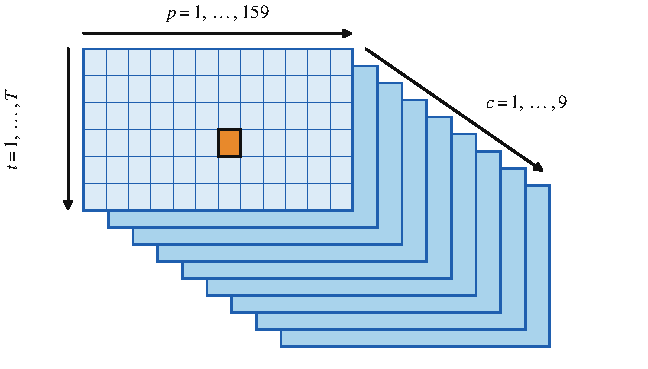
\includegraphics[width=\linewidth]{figures/tensor.pdf}
\sidecaption{Tensor $X\in\R^{T\times9\times159}$ jako stos dziewięciu macierzy (kanałów); przedni płat ($c=1$) ma narysowaną siatkę: $T$ wierszy (oś $t$, w dół) i $159$ kolumn (oś $p$, poziomo), a kolejne kanały leżą za nim (oś $c$).
Pomarańczowa kratka to jeden element $X_{t,c,p}$; trzy indeksy jednoznacznie wskazują jedną liczbę. \label{rys:tensor}}
\end{figure}

\begin{pulapka}
Kształt $(T,C,P)$ i kształt $(C,T,P)$ to dwa różne tensory, nawet gdy mają tyle samo liczb. W kodzie PyTorch
sieć dostaje tensor $[B,C,T,P]$ (paczka, kanały, czas, biny), a cechy zapisujemy jako $[T,C,P]$. Zawsze
sprawdzaj kształt przed operacją; błąd w kolejności osi daje poprawnie działający program z bezsensownym wynikiem.
\end{pulapka}

\section{Funkcje i ich składanie}

\haslo{złożenie funkcji}
\begin{definicja}[Funkcja i złożenie]\label{def:zlozenie}
\emph{Funkcja} $f\colon A\to B$ przypisuje każdemu elementowi zbioru $A$ dokładnie jeden element zbioru $B$.
\emph{Złożeniem} funkcji $f\colon A\to B$ i $g\colon B\to C$ jest funkcja $g\circ f\colon A\to C$,
$(g\circ f)(x)=g(f(x))$.
\end{definicja}

\begin{przyklad}\label{prz:zlozenie}
Niech $f(x)=2x$ i $g(x)=x+3$. Wtedy $(g\circ f)(5)=g(10)=13$, a $(f\circ g)(5)=f(8)=16$. Kolejność ma znaczenie:
złożenie nie jest przemienne.
\end{przyklad}

\begin{intuicja}
Cały model Gen~6 to jedno długie złożenie $\mathrm{model}=f_n\circ\dots\circ f_2\circ f_1$: cechy wchodzą do
pierwszej warstwy, jej wynik do drugiej itd. W rozdziale~\ref{rozdz:opis} rozpiszemy je w całości.
Dlatego ważne jest, by każda warstwa miała jasno określone wejście i wyjście: ich kształty muszą do siebie pasować.
\end{intuicja}

\begin{figure}[ht]
\centering
\begin{tikzpicture}[>=Stealth,node distance=0.85cm,blok/.append style={minimum width=12mm}]
  \node[blok] (x) {$\vect x$};
  \node[blok,right=of x] (f1) {$f_1$};
  \node[blok,right=of f1] (f2) {$f_2$};
  \node[blok,right=of f2] (f3) {$f_3$};
  \node[blok,right=of f3] (y) {$\vect y$};
  \draw[wektor] (x)--(f1); \draw[wektor] (f1)--(f2); \draw[wektor] (f2)--(f3); \draw[wektor] (f3)--(y);
  \node[font=\footnotesize,above=0.5mm of $(x.east)!0.5!(f1.west)$] {$\R^{n_0}$};
  \node[font=\footnotesize,above=0.5mm of $(f1.east)!0.5!(f2.west)$] {$\R^{n_1}$};
  \node[font=\footnotesize,above=0.5mm of $(f2.east)!0.5!(f3.west)$] {$\R^{n_2}$};
  \node[font=\footnotesize,above=0.5mm of $(f3.east)!0.5!(y.west)$] {$\R^{n_3}$};
\end{tikzpicture}
\sidecaption{Złożenie trzech funkcji $\vect y=f_3(f_2(f_1(\vect x)))$. Nad strzałkami stoją przestrzenie, w których
żyje wynik każdego kroku; wyjście jednej funkcji musi mieć kształt wejścia następnej. \label{rys:zlozenie}}
\end{figure}

\section{Potęgi i logarytm}

Wysokość dźwięku, głośność w decybelach i położenie binu na osi częstotliwości są w tej książce mierzone
\emph{logarytmicznie}. Powód zobaczymy w rozdziale~\ref{rozdz:dzwiek}; tu przypominamy narzędzie.

\haslo{logarytm}
\begin{definicja}[Logarytm]\label{def:log}
Dla $b>0$, $b\neq1$ i $x>0$ \emph{logarytmem} $\log_b x$ nazywamy jedyną liczbę $y$, dla której $b^{y}=x$.
Logarytm przy podstawie $e$ oznaczamy $\ln x$, a przy podstawie $10$ po prostu $\log_{10}x$.
\end{definicja}

\begin{przyklad}\label{prz:log}
$\log_2 8=3$, bo $2^3=8$. $\log_2\tfrac12=-1$, bo $2^{-1}=\tfrac12$. $\log_2 3\approx1{,}585$, bo
$2^{1{,}585}\approx3$. Logarytmu z liczby niedodatniej nie ma, bo żadna potęga liczby dodatniej nie jest
ujemna ani zerowa.
\end{przyklad}

\begin{twierdzenie}[Logarytm iloczynu]\label{tw:log-iloczynu}
Dla $x,y>0$ zachodzi $\log_b(xy)=\log_b x+\log_b y$ oraz $\log_b(x^{k})=k\log_b x$ dla każdej liczby rzeczywistej $k$.
\end{twierdzenie}
\begin{pomyslDowodu}
Zamieniamy $x$ i $y$ na potęgi podstawy $b$ i dodajemy wykładniki.
\end{pomyslDowodu}
\begin{proof}
Niech $u=\log_b x$ i $v=\log_b y$, czyli $x=b^{u}$ i $y=b^{v}$. Wtedy
\begin{align*}
xy &= b^{u}b^{v}=b^{u+v} && \pow{(wykładniki się dodają)}\\
\log_b(xy) &= u+v=\log_b x+\log_b y && \pow{(def.~\ref{def:log})}
\end{align*}
Dla potęgi: $x^{k}=(b^{u})^{k}=b^{uk}$, więc $\log_b(x^{k})=uk=k\log_b x$.
\end{proof}

Zdanie ludzkim językiem: logarytm zamienia \emph{mnożenie} na \emph{dodawanie}. Mnożenie częstotliwości
przez $2$ (oktawa wyżej) staje się dodaniem stałej $1$ do $\log_2 f$, bez względu na to, od jakiej
częstotliwości zaczynamy (\cref{rys:os-log}b). To jest sedno całej książki.

\begin{figure*}[ht]
\centering
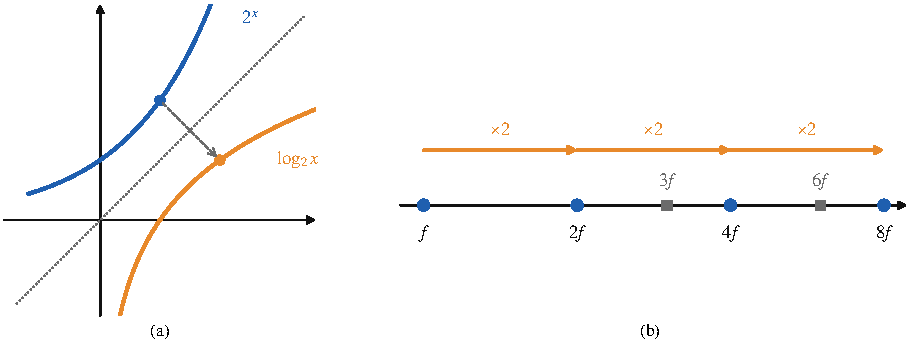
\includegraphics[width=\linewidth]{figures/os-log.pdf}
\caption{(a) Funkcje $2^x$ (niebieska) i $\log_2 x$ (pomarańczowa) są swoimi lustrzanymi odbiciami względem
prostej $y=x$ (kropkowana): odbicie punktu $(2,4)$ to $(4,2)$. (b) Na osi logarytmicznej kolejne podwojenia
$f,2f,4f,8f$ leżą w równych odstępach (pomarańczowe strzałki mają tę samą długość); punkty $3f$ i $6f$ też
dzieli dokładnie jeden taki krok, bo $\log_2 6-\log_2 3=1$.}
\label{rys:os-log}
\end{figure*}

\begin{naliczbach}
Ile wynosi $\log_2 12$? Zapisujemy $12=3\cdot 2^2$ i stosujemy twierdzenie~\ref{tw:log-iloczynu}:
$\log_2 12=\log_2 3+2\log_2 2=1{,}585+2=3{,}585$. Sprawdzenie: $2^{3{,}585}\approx 12{,}0$.
Ta sztuczka (rozbicie na iloczyn znanych czynników) pozwoli nam w rozdziale~\ref{rozdz:alikwoty} policzyć, ile półtonów
leży nad daną nutą jej trzeci alikwot.
\end{naliczbach}

\begin{twierdzenie}[Zmiana podstawy]\label{tw:zmiana-podstawy}
Dla $a,b>0$, $a,b\neq1$ i $x>0$ zachodzi $\log_b x=\dfrac{\log_a x}{\log_a b}$.
\end{twierdzenie}
\begin{pomyslDowodu}
Logarytmujemy obie strony równości $x=b^{\log_b x}$ przy podstawie $a$.
\end{pomyslDowodu}
\begin{proof}
Niech $y=\log_b x$, czyli $x=b^{y}$. Stosujemy $\log_a$ do obu stron:
\begin{align*}
\log_a x &= \log_a\!\big(b^{y}\big) && \pow{(podstawienie)}\\
         &= y\,\log_a b && \pow{(tw.~\ref{tw:log-iloczynu})}\\
\Rightarrow\; y &= \frac{\log_a x}{\log_a b}. && \pow{(dzielimy przez $\log_a b\neq0$)}
\end{align*}
Ponieważ $y=\log_b x$, to jest dokładnie dowodzony wzór.
\end{proof}

W praktyce: kalkulator ma zwykle tylko $\ln$ i $\log_{10}$, więc $\log_2 x=\ln x/\ln 2$. W programie \texttt{np.log2(x)}
daje to samo.

\section{Funkcje pomocnicze}

W modelu pojawi się kilka prostych funkcji, które warto poznać od razu.

\begin{figure*}[ht]
\centering
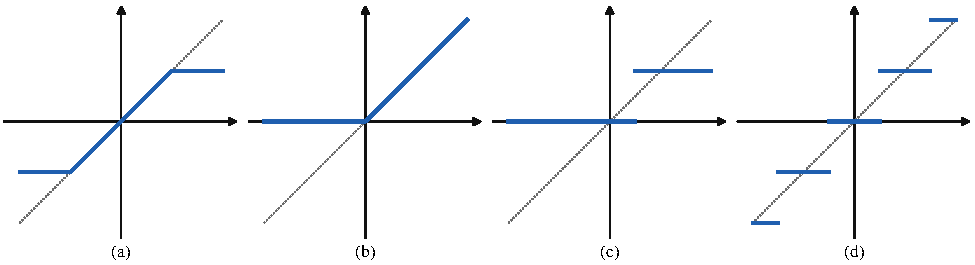
\includegraphics[width=\linewidth]{figures/funkcje-pomocnicze.pdf}
\caption{Cztery proste funkcje jednej zmiennej na tle prostej $y=x$ (kropkowana). (a) $\clip(x,-1,1)$ przycina wartości do przedziału.
(b) $\max(0,x)$, czyli $\ReLU$, zeruje wartości ujemne. (c) Wskaźnik $\indic{x\ge\frac12}$ jest równy $1$ albo $0$. (d) $\round(x)$ zaokrągla do najbliższej całkowitej.
Funkcje (c) i (d) mają skoki, więc nie da się ich używać w uczeniu przez gradient; dlatego dekoder w rozdziale~\ref{rozdz:dekoder} jest poza siecią.}
\label{rys:funkcje-pomocnicze}
\end{figure*}

\begin{center}\small
\begin{tabular}{@{}p{2.6cm}p{4.4cm}p{3.9cm}@{}}
\toprule
zapis & znaczenie & przykład\\
\midrule
$\clip(x,a,b)$ & $\min(\max(x,a),b)$ & $\clip(1{,}7;0;1{,}3)=1{,}3$\\
$\max_i a_i$ & największa z liczb & $\max(2,5,3)=5$\\
$\argmax_i a_i$ & \emph{numer} największej & $\argmax(2,5,3)=2$ (od 1)\\
$\indic{\text{warunek}}$ & $1$, gdy prawda, inaczej $0$ & $\indic{3>2}=1$\\
$\round(x)$ & najbliższa całkowita & $\round(35{,}07)=35$\\
$\lfloor x\rfloor$ & część całkowita w dół & $\lfloor 2{,}9\rfloor=2$\\
\bottomrule
\end{tabular}
\end{center}

\begin{pulapka}
$\argmax$ zwraca \emph{miejsce}, a $\max$ \emph{wartość}. Pomylenie ich jest tak częste, że w kodzie dekodera
(rozdział~\ref{rozdz:dekoder}) wybór struny to $\argmax$ po strunach, a pewność nuty to $\max$.
\end{pulapka}

\section*{Podsumowanie}
\begin{itemize}
\item Suma $\sum$ to pętla dodająca; stałą wolno wyciągnąć przed sumę (tw.~\ref{tw:liniowosc-sumy}).
\item Tensor to tablica liczb o kształcie $(n_1,\dots,n_r)$; cechy modelu to $X\in\R^{T\times9\times159}$.
\item Model to złożenie funkcji; kształty wyjść i wejść muszą do siebie pasować.
\item Logarytm zamienia mnożenie na dodawanie, a podwojenie częstotliwości na stały krok (tw.~\ref{tw:log-iloczynu}).
\item $\clip$, $\max$, $\argmax$, wskaźnik i zaokrąglenie to cegiełki dekodera i normalizacji cech.
\end{itemize}

\begin{sprawdz}
\begin{enumerate}
\item Policz $\sum_{i=1}^{5}(2i-1)$ i podaj wynik w prostszej postaci. (Wskazówka: tw.~\ref{tw:liniowosc-sumy} oraz $\sum i = n(n+1)/2$.)
\item Ile liczb ma tensor kształtu $[16,\,9,\,192,\,159]$ (paczka 16 wycinków po 192 klatki)? Ile to megabajtów w formacie \texttt{float16} (2 bajty na liczbę)?
\item Policz $\log_2 48$ i $\log_2\sqrt2$ bez kalkulatora, znając $\log_2 3\approx1{,}585$.
\item Czy $\log_b(x+y)=\log_b x+\log_b y$? Podaj kontrprzykład liczbowy.
\end{enumerate}
\end{sprawdz}

\subsection*{Rozwiązania}
\begin{enumerate}
\item $\sum_{i=1}^5(2i-1)=2\cdot15-5=25$ (suma pierwszych $n$ nieparzystych to $n^2$); sprawdzenie: $1+3+5+7+9=25$.
\item $16\cdot9\cdot192\cdot159=4\,396\,032$ liczb, czyli $\approx 8{,}8$~MB w \texttt{float16}.
\item $48=3\cdot2^4$, więc $\log_2 48=1{,}585+4=5{,}585$; $\log_2\sqrt2=\tfrac12$.
\item Nie. Dla $b=2$ i $x=y=4$ mamy $\log_2(4+4)=\log_2 8=3$, a $\log_2 4+\log_2 4=2+2=4$. Prawdziwy jest wzór na \emph{iloczyn}: $\log_2(4\cdot4)=\log_2 16=4$.
\end{enumerate}
